\documentclass{article}

\usepackage{fullpage}
\usepackage{url}
\usepackage{graphicx}
\usepackage{amsmath}
\usepackage{physics}
\usepackage{mathtools}
\usepackage{bbold}

\DeclareMathOperator{\erfi}{erfi}
\newcommand{\R}{\ensuremath{\mathbb{R}}}
\newcommand{\C}{\ensuremath{\mathbb{C}}}

\title{Quantum Mechanics I Test}
\author{Idan Stark}
\date{\today}

\begin{document}
\maketitle
I selected question 2
\section{The Born-Oppenheimer approximation}
We consider the hamiltonian\footnote{Notice! (more to myself then anything) It can be confusing that $k$ here doesn't have anything to do with the wave number/momentum. In terms of units $k \propto \omega^2 \propto k_\omega^4$.}
\begin{equation}
    H = \frac{p_x^2}{2m} + \frac{p_y^2}{2M} + \frac{k\left(x^2 + y^2\right)}{2} + \alpha xy
\end{equation}
Going forward, we write
\begin{equation}
    H = H_0 + h
\end{equation}
where
\begin{equation}
    H_0 = \frac{p_y^2}{2M} + \frac{k}{2}y^2
    \qquad
    h = \frac{p_x^2}{2m} + \frac{k}{2}x^2 + \alpha xy
\end{equation}
\subsection{Solution using the BO approximation}
\subsubsection{The adiabatic basis}
Let us start by finding the adiabatic basis (redfined as per the BO approximation method):
\begin{equation}
    h(x; y) \phi_n(x; y) = \epsilon_n(y)\phi_n(x;y)
\end{equation}
For this let us change to a variable:
\begin{equation}
    z = x + \frac{\alpha}{k} y
    \qquad \rightarrow \qquad
    \frac{k}{2}z^2 =\frac{k}{2}x^2 + \alpha x y + \frac{\alpha^2}{2k}y^2
\end{equation}
Which means:
\begin{equation}
    h(z; y) = \frac{p_z^2}{2m} + \frac{k}{2}z^2 - \frac{\alpha^2y^2}{2k}
\end{equation}
Which is just a harmonic oscillator with an additional constant. So, the energy levels are:
\begin{equation}
    \phi_n(x; y) = \phi_n^{h.o.}\left(x + \frac{\alpha}{k} y\right)
    \qquad
    \epsilon_n(y) = \epsilon_n^{h.o.} - \frac{\alpha^2y^2}{2k}
\end{equation}
Where $\phi_n^{h.o.}$ are the harmonic oscillator eigenfunctions and $\epsilon_n^{h.o.}$ eigenenergies. Let us note that the energies depend on the frequency, which in this case is:
\begin{equation}
    \omega_x = \sqrt{\frac{k}{m}}
\end{equation}
The adiabatic energy levels can be seen in figure 1.
\begin{figure}[h]
    \centering
    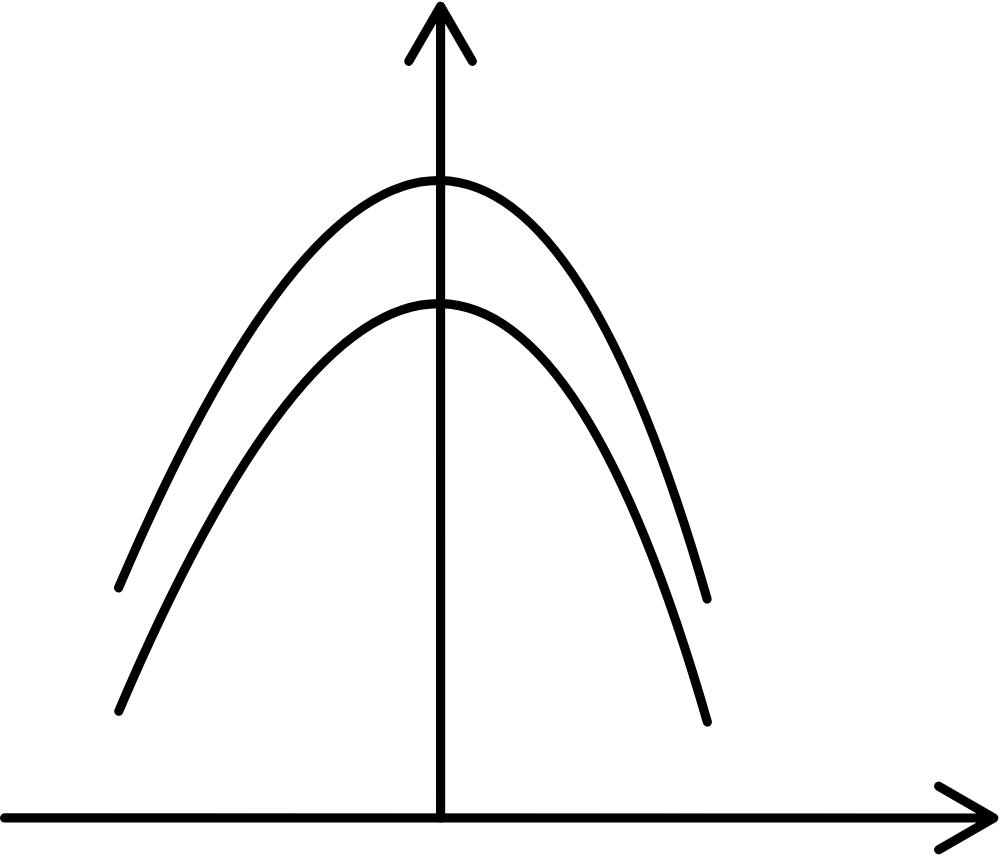
\includegraphics[width=0.6\textwidth]{Notewise-Untitled 2025-12-30-20260215173001.png}
    \caption{Adiabadic energy levels $\epsilon_{n}(y)$ as a function of $y$}
\end{figure}
\subsubsection{The Berry phase}
Next, let us look at the Berry phase of these energy levels:
\begin{equation}
    \gamma_n(y) = \int_0^y dy' \bra{\phi_n} \frac{\partial}{\partial_y} \ket{\phi_n}
\end{equation}
But, since $\phi_n^{h.o.}$ are real, and the berry phase is pure imaginary, it must be zero. This can also be seen by differntiating by hand. The harmonic oscillator eigenfunctions are`':
\begin{equation}
    \phi_n^{h.o.}(z) = A \frac{(-1)^n}{\sqrt{2^n n!}} \left(\frac{\partial}{\partial z}\right)^n e^{-z^2 / l^2}
\end{equation}
Where $A$ is the noramlizaiton constant and $l = \sqrt{\frac{\hbar}{m\omega}}$ is the length scale. As can be easily seen, the derivative is simply the next level:
\begin{equation}
    \frac{\partial}{\partial y} \phi_n^{h.o.}(z(x, y)) = 
    \frac{\partial z}{\partial y} \frac{\partial}{\partial z} \phi_n^{h.o.}(z) = \frac{\alpha}{k} \phi_{n+1}^{h.o.}(z)
\end{equation}
Which means:
\begin{equation}
    \bra{\phi_n} \partial_y \ket{\phi_n} \propto \braket{\phi_n}{\phi_{n+1}} = 0
\end{equation}
And so the Berry phase is zero. Actually, not only is Berry phase zero, but also the Berry connection and the Berry curvature. This hints at something that should be clear from the dimensionality of the problem and the shapes of the energy levels - there are no energy level crossings. If there were level crossings, they would act as magnetic monopoles for the Berry connection in the parameter space, and it would be non-zero everywhere.
\newline
We can see the same fact from the dimensionality of the system: for a real values hamiltonian, the required number of parameters for a level crossing is $M = 2$, in which case the energy levels would meet at a single point. Any less variables then that and there isn't even a single point of crossing. Lastly, this can be seen from the actual structure of the energy levels, being seperated by a constant $\hbar \omega$ for every value of $y$.
\subsubsection{The slow Degree of Freedom}
We can now write the solution for the entire porblem in the adiabatic basis:
\begin{equation}
\label{eq:total1}
    \Psi(x, y) = \sum_n \xi_n(y) \phi_n(x, y)
\end{equation}
The Born-Oppenheimer approximation tells us that for a hamiltonian of the form
\begin{equation}
    H_0 = \frac{p_y^2}{2M} + U(y)
\end{equation}
The equations for the coefficients $\xi(y)$ is given by:
\begin{equation}
    \frac{1}{2M}\left[p_y - A_m(y)\right]^2\xi_m(y) + \left[U(y) + \epsilon_m(y)\right]\xi_m(y) = E \xi_m(y)
\end{equation}
Where $A_m$ is the Berry connection and $E$ is the total energy. But, since the Berry connection is zero, we can write (writing the actual potential $U(y)$ and the energy level $\epsilon_n(y)$ as well):
\begin{equation}
    \frac{p_y^2}{2M}\xi_m(y) + \left[\frac{k}{2}y^2 + \epsilon_m^{h.o.} - \frac{\alpha^2y^2}{2k}\right]\xi_m(y) = E \xi_m(y)
\end{equation}
Which gives:
\begin{equation}
    \left[\frac{p_y^2}{2M} + \frac{k^2 - \alpha^2}{2k}y^2\right]\xi_m(y) = \left(E - \epsilon_m^{h.o.}\right) \xi_m(y)
\end{equation}
This is again a harmonic oscillator, this time with frequency
\begin{equation}
    \omega_y = \sqrt{\frac{k^2 - \alpha^2}{kM}}
\end{equation}
This gives the solutions for the coefficients as variables of the slow variable $y$:
\begin{equation}
    \xi_n(y) = \phi_n^{h.o.}(y;\omega_y)
\end{equation}
\subsubsection{Bringing it all together}
So, we can write the eigenfunctions for the entire system with the two quantum numbers $n_y$ and $n_x$ and based on equation \ref{eq:total1}:
\begin{equation}
    \Psi_{n_y,n_x} (x, y) = \xi_{n_y}(y) \phi_{n_x}(x, y) = \phi_{n_y}^{h.o.}(y;\omega_y)  \phi_{n_x}^{h.o.}\left(x + \frac{\alpha}{k} y; \omega_x\right)
\end{equation}
With the energies:
\begin{equation}
    E_{n_y,n_x} = \epsilon_{n_y}(\omega_y) + \epsilon_{n_x}(\omega_x) = \hbar\omega_y\left(n_y + \frac{1}{2}\right) + \hbar\omega_x\left(n_x + \frac{1}{2}\right)
\end{equation}
\begin{equation}
    E_{n_y,n_x} = \hbar\left[\sqrt{\frac{k^2 - \alpha^2}{kM}}\left(n_y + \frac{1}{2}\right) + \sqrt{\frac{k}{m}}\left(n_x + \frac{1}{2}\right)\right]
\end{equation}
\subsubsection{Seperation of variables}
The Born-Oppenheimer approximation is based on a "fake" seperation of variables. We "freeze" one variable as a constant, solve the other one, and then use those solutions to unfreeze the original variable. For this reason, the above solution acts very much like two independent harmonic oscillators. Because of this, the coupling constant $\alpha$ appears only in specific interations. In the eigenenergies, it affects only by reducing the y-dependent energy, while in the eigenfunctions it affects only by changing the shape of the x-dependent part.
\newline
Taking $\alpha \rightarrow 0$ will give two independent harmonic oscillators with frequency $\omega_{x,y} = \sqrt{\frac{k}{m}}, \sqrt{\frac{k}{M}}$.

\subsection{Exact Solution}
Now let us find the exact solution. For this, let us find a transformation to a set of coordinates $(s, t)$ in which the hamiltonian is diagonable:
\begin{equation}
    \begin{pmatrix}
        x \\ y
    \end{pmatrix} = \begin{pmatrix}
        a & b \\ c & d
    \end{pmatrix} \begin{pmatrix}
        s \\ t
    \end{pmatrix}
\end{equation}
And the inverse:
\begin{equation} \begin{pmatrix}
        s \\ t
    \end{pmatrix} = \frac{1}{|ad - bc|}\begin{pmatrix}
        d & -b \\ -c & a
    \end{pmatrix}
    \begin{pmatrix}
        x \\ y
    \end{pmatrix}
\end{equation}
And through coordinates scaling, let us choose coordinates such that the determinant is $\pm 1$:
\begin{equation} \begin{pmatrix}
        s \\ t
    \end{pmatrix} = \begin{pmatrix}
        d & -b \\ -c & a
    \end{pmatrix}
    \begin{pmatrix}
        x \\ y
    \end{pmatrix}
\end{equation}
The momenta then act like derivatives, i.e. changing according to the inverse:
\begin{equation}
    \partial_x = \frac{\partial s}{\partial x} \partial_s + \frac{\partial t}{\partial x} \partial_t = d \partial_s - c\partial_t
\end{equation}
So:
\begin{equation}
    \begin{pmatrix}
        p_x \\ p_y
    \end{pmatrix} = \begin{pmatrix}
        \frac{\partial s}{\partial x} & \frac{\partial t}{\partial x} \\ \frac{\partial s}{\partial y} & \frac{\partial t}{\partial y}
    \end{pmatrix} \begin{pmatrix}
        p_s \\ p_t
    \end{pmatrix} = \begin{pmatrix}
        d & -c \\ -b & a
    \end{pmatrix} \begin{pmatrix}
        p_s \\ p_t
    \end{pmatrix}
\end{equation}
Now, the hamiltonian can be written as
\begin{equation}
\begin{gathered}
    H = \frac{p_x^2}{2m} + \frac{p_y^2}{2M} + \frac{k\left(x^2 + y^2\right)}{2} + \alpha xy = \\ =
    \frac{(dp_s - cp_t)^2}{2m} + \frac{(ap_t - b p_s)^2}{2M} + \frac{k}{2}\left((as + bt)^2 + (cs + dt)^2\right) + \alpha(as + bt)(cs + dt) = \\ =
    \left(d^2 + \frac{m}{M}b^2\right)\frac{p_s^2}{2m}
    + \left(c^2 + \frac{m}{M}a^2\right)\frac{p_t^2}{2m}
    - 2\left(cd + \frac{m}{M}ab\right)\frac{p_s p_t}{2m}
    + \\ + \left(\frac{k(a^2 + c^2)}{2} + \alpha a c\right)s^2
    + \left(\frac{k(b^2 + d^2)}{2} + \alpha bd\right)t^2
    + \left(k(ab + cd) + \alpha (ad + bc)\right)st
\end{gathered}
\end{equation}
We are looking for a transformation that has no interaction, so:
\begin{equation}
    cd + \frac{m}{M}ab = 0
    \qquad
    k(ab + cd) + \alpha (ad + bc) = 0
\end{equation}
Pluggin the first equation into the second gives:
\begin{equation}
    k\left(1 - \frac{m}{M}\right)ab + \alpha \left(ad + \frac{m}{M}\frac{ab^2}{c}\right) = 0
\end{equation}
Assuming $a \ne 0$:
\begin{equation}
    k\left(1 - \frac{m}{M}\right)b + \alpha \left(d + \frac{m}{M}\frac{b^2}{c}\right) = 0
\end{equation}
\begin{equation}
    d = - \frac{1}{\alpha}\left(kb + \frac{m}{M}\left(\alpha\frac{b^2}{c}- kb\right)\right)
\end{equation}
So, a convinient solution would be:
\begin{equation}
    c = \frac{\alpha}{k}b
    \qquad
    d = -\frac{k}{\alpha}b
\end{equation}
Now, plugging that back into the first equations gives:
\begin{equation}
    a = \frac{M}{m}b
\end{equation}
Finally, let us require that $\det = \pm1$:
\begin{equation}
    ad - bc = \left(-\frac{M}{m}\frac{k}{\alpha} - \frac{\alpha}{k}\right)b^2 = \pm1
    \rightarrow
    b = \sqrt{\frac{mk\alpha}{Mk^2 + m\alpha^2}}
\end{equation}
Where we chose the sign based on the sign of $k\alpha$. So the final values are:
\begin{equation}
    \begin{pmatrix}
        a & b \\ c & d
    \end{pmatrix} = \sqrt{\frac{mk\alpha}{Mk^2 + m\alpha^2}}\begin{pmatrix}
        \frac{M}{m} & 1 \\ \frac{\alpha}{k} & -\frac{k}{\alpha}
    \end{pmatrix}
\end{equation}
Which makes the hamiltonian
\begin{equation}
\begin{gathered}
    H =
    \frac{mk\alpha}{Mk^2 + m\alpha^2}\left[
        \left(\frac{k^2}{\alpha^2} + \frac{m}{M}\right)\frac{p_s^2}{2m}
        + \left(\frac{\alpha^2}{k^2} + \frac{M}{m}\right)\frac{p_t^2}{2m}
        + \frac{k}{2}\frac{M}{m}\left(\frac{M}{m} + 3\frac{\alpha^2}{k^2}\right)s^2
        + \frac{k}{2}\left(\frac{k^2}{\alpha^2} - 1\right)t^2
    \right] = \\ =
    \frac{k}{\alpha}\frac{p_s^2}{2M}
    + \frac{\alpha}{k}\frac{p_t^2}{2m} +
    \frac{mk\alpha}{Mk^2 + m\alpha^2}\left[
        \frac{k}{2}\frac{M}{m}\left(\frac{M}{m} + 3\frac{\alpha^2}{k^2}\right)s^2
        + \frac{k}{2}\left(\frac{k^2}{\alpha^2} - 1\right)t^2
    \right]
\end{gathered}
\end{equation}
And we got the hamiltonian for two decoupled harmonic oscillators.
The solutions to which are:
\begin{equation}
    \ket{n_s, n_t} = \phi_{n_s}^{h.o.}\left(s; \omega_s\right)\phi_{n_t}^{h.o.}\left(t;\omega_t\right)
\end{equation}
And the eigenenergies are
\begin{equation}
    E_{n_s, n_t} = \hbar\omega_s \left(n_s + \frac{1}{2}\right) + \hbar\omega_t \left(n_t + \frac{1}{2}\right)
\end{equation}
Where
\begin{equation}
    \omega_s = \sqrt{\frac{k}{2M}\frac{mk^2}{Mk^2 + m\alpha^2}\frac{M}{m}\left(\frac{M}{m} + 3\frac{\alpha^2}{k^2}\right)}
    \qquad
    \omega_t = \sqrt{\frac{k}{2}\frac{1}{Mk^2 + m\alpha^2}\left(k^2 - \alpha^2\right)}
\end{equation}
This is probably not the simplest solution to the decoupling of the hamiltonian, but it shows the relation to the OB approximation. For start, when $\alpha \rightarrow 0$, we get the same decoupled harmonic oscillators as the matrix becomes diagonal and the frequencies collapse to their previous form.
\newline
Additionaly, in contrast to the BO solution, the interaction effects on each of the coordinates in both the solution and the energy levels. This is a because in this form we did not "freeze" one of the variables while solving the other, forcing the assymetry between the variables (notice that in this solution $M$ and $m$ are interchangable, while this is not so in the OB solution for obvious reasons).
\end{document}